\documentclass{article}%
\usepackage[T1]{fontenc}%
\usepackage[utf8]{inputenc}%
\usepackage{lmodern}%
\usepackage{textcomp}%
\usepackage{lastpage}%
\usepackage{geometry}%
\geometry{margin=2cm}%
\usepackage{graphicx}%
\usepackage{ragged2e}%
%
%
%
\begin{document}%
\normalsize%
\begin{minipage}{0.6\linewidth}%
\begin{flushleft}%
\large{Course: \textbf{New Course}}%
\vspace{0.1cm}%
\newline%
\vspace{0.1cm}%
\normalsize{Professor: \textbf{New Prof}}%
\newline%
\vspace{0.1cm}%
\normalsize{\textbf{Theoretical} assignment}%
\end{flushleft}%
\end{minipage}%
\begin{minipage}{0.36\linewidth}%
\begin{flushright}%

\includegraphics[width=1.75cm]{logo.png}%
\hfill%
\newline%
\hfill%
\textbf{\normalsize{Sharif University of Technology}}%
\end{flushright}%
\end{minipage}%
\begin{center}%
\hrule height 0.02cm%
\vspace{0.2cm}%
\large{\textbf{New Assignment}}%
\vspace{0.2cm}%
\hrule height 0.02cm%
\end{center}%
\section{\textbf{Cache Memory Hierarchy}}%
\label{sec:textbfCacheMemoryHierarchy}%
The concept of a memory hierarchy is integral to computer architecture, illustrating the various levels of memory and their roles in storing and providing access to data. At the pinnacle of this hierarchy resides the cache memory, an essential component strategically positioned to facilitate expeditious data retrieval and enhance system performance. 

## Question: 

### Part 1: 

Explain the concept of a memory hierarchy, its purpose, and the unique position cache memory occupies within this structure. Elaborate on the following: 

- The strategic placement of cache memory within the hierarchy and its proximity to the processor. 

- How cache memory interacts with other memory levels, such as main memory and secondary storage. 

### Part 2: 

Provide a diagram illustrating the memory hierarchy, clearly depicting the following: 

- The various levels of the hierarchy, including cache memory, main memory, and secondary storage. 

- The flow of data between the processor and different memory levels, highlighting cache memory's role as a high-speed intermediary. 

### Part 3: 

Discuss the design considerations for optimizing cache performance, taking into account the following factors: 

- Cache size and its impact on hit rate and system speed. 

- Cache organization, including direct-mapped, fully associative, and set-associative caches, and the trade-offs between them. 

- Replacement policies, such as Least Recently Used (LRU), and their influence on cache efficiency. 

- Write policies, including write-back and write-through, and their implications for data consistency and system performance. 

Provide specific examples and analyses to substantiate your explanations, ensuring a comprehensive understanding of cache memory's role and the design choices that influence its performance within the memory hierarchy.%
\begin{center}%
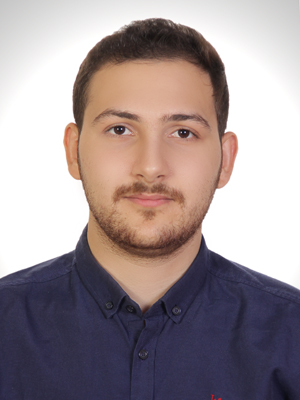
\includegraphics[width=8cm]{./questionattachments/46993.jpg}%
\end{center}

%
\section{\textbf{teest}}%
\label{sec:textbfteest}%
## Cache Performance Analysis and Comparison

### Part 1: Analysis of Cache Performance
Analyze and compare the performance of direct-mapped and fully associative caches. Consider parameters such as hit rate, miss rate, and average access time in your analysis. 

### Part 2: Recommendation for High-Performance Computing
Present your findings from Part 1 and explain which cache organization you would recommend for a system with an emphasis on high-performance computing. Be sure to justify your choice based on the analysis results.%
\begin{center}%
\includegraphics[width=8cm]{./questionattachments/SAT\_Poster\_dgTs8F5.png}%
\end{center}

%
\section{\textbf{test new Q}}%
\label{sec:textbftestnewQ}%
[Question]

---

## Part 1: 

Remove personally identifiable information and format the question. 

## Part 2: 

Please provide the anonymized and formatted question below: 

"A new and improved test question is presented for your attention."

%
\section{\textbf{Cache Performance}}%
\label{sec:textbfCachePerformance}%
## Cache Performance Analysis and Comparison

### Part 1: Analysis of Cache Performance
Analyze and compare the performance of direct-mapped and fully associative caches. Consider parameters such as hit rate, miss rate, and average access time in your analysis. 

### Part 2: Recommendation for High-Performance Computing
Present your findings from Part 1 and explain which cache organization you would recommend for a system with an emphasis on high-performance computing. Be sure to justify your choice based on the analysis results.%
\begin{center}%
\includegraphics[width=8cm]{./questionattachments/SAT\_Poster.png}%
\end{center}

%
\section{\textbf{cache fifo lifo}}%
\label{sec:textbfcachefifolifo}%
## Cache Performance Analysis and Comparison

### Part 1: Analysis of Cache Performance
Analyze and compare the performance of direct-mapped and fully associative caches. Consider parameters such as hit rate, miss rate, and average access time in your analysis. 

### Part 2: Recommendation for High-Performance Computing
Present your findings from Part 1 and explain which cache organization you would recommend for a system with an emphasis on high-performance computing. Be sure to justify your choice based on the analysis results.

%
\end{document}